\documentclass[a4paper,12pt]{article}
\usepackage[utf8]{inputenc}
\usepackage[spanish]{babel}
\usepackage{color}
\usepackage{parskip}
\usepackage{graphicx}
\usepackage{multirow}
\usepackage{listings}
\usepackage{vmargin}
\graphicspath{ {imagenes/} }
\definecolor{mygreen}{rgb}{0,0.6,0}
\definecolor{lbcolor}{rgb}{0.9,0.9,0.9}
\usepackage{epstopdf}


\setpapersize{A4}
\setmargins{2.5cm}       % margen izquierdo
{1.5cm}                        % margen superior
{16.5cm}                      % anchura del texto
{23.42cm}                    % altura del texto
{10pt}                           % altura de los encabezados
{1cm}                           % espacio entre el texto y los encabezados
{0pt}                             % altura del pie de página
{2cm}     

\lstset{
%backgroundcolor=\color{lbcolor},
    tabsize=4,    
%   rulecolor=,
    language=[GNU]C++,
        basicstyle=\tiny,
        aboveskip={1.5\baselineskip},
        columns=fixed,
        showstringspaces=false,
        extendedchars=false,
        breaklines=true,
        prebreak = \raisebox{0ex}[0ex][0ex]{\ensuremath{\hookleftarrow}},
        frame=single,
        showtabs=false,
        showspaces=false,
        showstringspaces=false,
        identifierstyle=\ttfamily,
        keywordstyle=\color[rgb]{0,0,1},
        commentstyle=\color[rgb]{0.026,0.112,0.095},
        stringstyle=\color{red},
        numberstyle=\color[rgb]{0.205, 0.142, 0.73},
%        \lstdefinestyle{C++}{language=C++,style=numbers}’.
}

\begin{document}
\begin{titlepage}

\begin{center}
\vspace*{-1in}

\begin{large}
UNIVERSIDAD NACIONAL DE SAN AGUSTÍN\\
\vspace*{0.15in}
ESCUELA PROFESIONAL DE CIENCIA DE LA COMPUTACIÓN\\
\end{large}
\begin{figure}[htb]
\centering
\includegraphics[scale=0.13]{/home/xnpio/Documentos/Caratula/logo.eps}
\end{figure}
\vspace*{0.15in}
\begin{large}
TEMA:\\
\end{large}
\vspace*{0.2in}
\begin{Large}
\textbf{QR ALGORITHM IN FORTRAN} \\
\end{Large}
\vspace{8mm}

\begin{large}
Curso:\\
\end{large}
\vspace*{0.2in}
\begin{Large}
\textbf{MATEMÁTICA APLICADA A LA COMPUTACIÓN} \\
\end{Large}

\vspace{8mm}

\begin{large}
\textbf{Presentado por:}\\

\begin{flushleft}

\hspace{7cm} Christofer Chávez Carazas \\

\end{flushleft}
\end{large}
\vspace{4cm}
\rule{80mm}{0.1mm}\\
\vspace*{0.1in}

\begin{large}
Arequipa - Perú \\
2017 \\
\end{large}
\end{center}
\end{titlepage}


 \twocolumn[]
 \section{Código}
 \begin{lstlisting}
  program qr
	integer :: n,iter
	real(16), dimension(3,3) :: A,Q,R,D
	n = 3

	call zeros(Q,n)
	call zeros(R,n)

	A(1,1) = 3
	A(1,2) = 8
	A(1,3) = 1

	A(2,1) = 2
	A(2,2) = 3
	A(2,3) = 8

	A(3,1) = 0
	A(3,2) = 2
	A(3,3) = 1

	iter = 10

	D = A
	do i = 1,iter
		call qrDesc(D,n,Q,R)
		call mulMatriz(R,Q,n,D)
		call printMatriz(D,n,n)
		call zeros(Q,n)
		call zeros(R,n)
		write(*,*)

	end do

end program qr

subroutine qrDesc(A,n,Q,R)
	integer :: n,i,j
	real(16), dimension(n,n) :: A,Q,R
	real(16), dimension(n) :: aTemp,eTemp,aeTemp,uTemp
	real(16), dimension(n) :: u
	real(16) :: numTemp,normTemp

	do i = 1,n
		call getCol(A,n,i,u)
		do j = 1,i
			call getCol(Q,n,j,eTemp)
			call getCol(A,n,i,aTemp)
			call mulList(aTemp,eTemp,n,numTemp)
			R(j,i) = numTemp
			call mulListNumber(eTemp,numTemp,n,aeTemp)
			call minusList(u,aeTemp,n,uTemp)
			u = uTemp
		end do
		call norm(u,n,normTemp)
		numTemp = 1.0 / normTemp
		call mulListNumber(u,numTemp,n,eTemp)
		call copyCol(eTemp,Q,n,i)
		call getCol(Q,n,i,eTemp)
		call getCol(A,n,i,aTemp)
		call mulList(aTemp,eTemp,n,numTemp)
		R(i,i) = numTemp
	end do

return
end subroutine qrDesc

subroutine getCol(A,n,k,res)
	integer :: n,k,i
	real(16), dimension(n,n) :: A
	real(16), dimension(n) :: res

	do i = 1,n
		res(i) = A(i,k)
	end do

return 
end subroutine getCol

subroutine mulList(A,B,n,res)
	integer :: n,i
	real(16) :: res
	real(16), dimension(n) :: A,B
	res = 0

	do i = 1,n
		res = res + (A(i) * B(i))
	end do

return
end subroutine mulList

subroutine mulListNumber(A,b,n,res)
	integer :: n,i
	real(16) :: b
	real(16), dimension(n) :: A,res

	do i = 1,n
		res(i) = A(i) * b
	end do

return
end subroutine mulListNumber

subroutine minusList(A,B,n,res)
	integer :: n,i
	real(16), dimension(n) :: A,B,res

	do i = 1,n
		res(i) = A(i) - B(i)
	end do

return
end subroutine minusList

subroutine norm(A,n,res)
	integer :: n,i
	real(16), dimension(n) :: A
	real(16) :: res
	res = 0

	do i = 1,n
		res = res + abs(A(i)) ** 2
	end do
	res = sqrt(res)

return
end subroutine norm

subroutine copyCol(A,B,n,k)
	integer :: n,i,k
	real(16), dimension(n,n) :: B
	real(16), dimension(n) :: A

	do i = 1,n
		B(i,k) = A(i)
	end do
return
end subroutine copyCol

subroutine mulMatriz(A,B,n,res)
	integer :: n,i,k,j
	real(16), dimension(n,n) :: A,B,res
	real(16) :: sumTemp
	do i = 1,n
		do j = 1,n
			sumTemp = 0
			do k = 1,n
				sumTemp = sumTemp + A(i,k) * B(k,j)
			end do
			res(i,j) = sumTemp
		end do
	end do
return
end subroutine mulMatriz

subroutine printMatriz(M,f,c)
	integer :: i,j
	integer :: f,c
	real(16), dimension(f,c) :: M
	do i=1,f
    	do j=1,c
        	write(*,'(F10.6,$)') M(i,j)
    	end do
    	write(*,*)
	end do
return
end subroutine printMatriz

subroutine zeros(A,n)
	integer :: n,i,j
	real(16), dimension(n,n) :: A
	do i = 1,n
		do j = 1,n
			A(i,j) = 0
		end do
	end do
return 
end subroutine zeros
 \end{lstlisting}

 \onecolumn
 
 \section{Ejemplo}
 
El ejemplo mostrado se realiza con la siguiente matriz:
 
  
 \[ A = \left[ \begin{array}{ccc}
3 & 8 & 1 \\
2 & 3 & 8 \\
0 & 2 & 1 \end{array} \right]\]

\textbf{Número de iteraciones:} $5$

\section{Resultados}

Se muestra el resultado de cada iteración.

\begin{figure} [h]
 \centering
 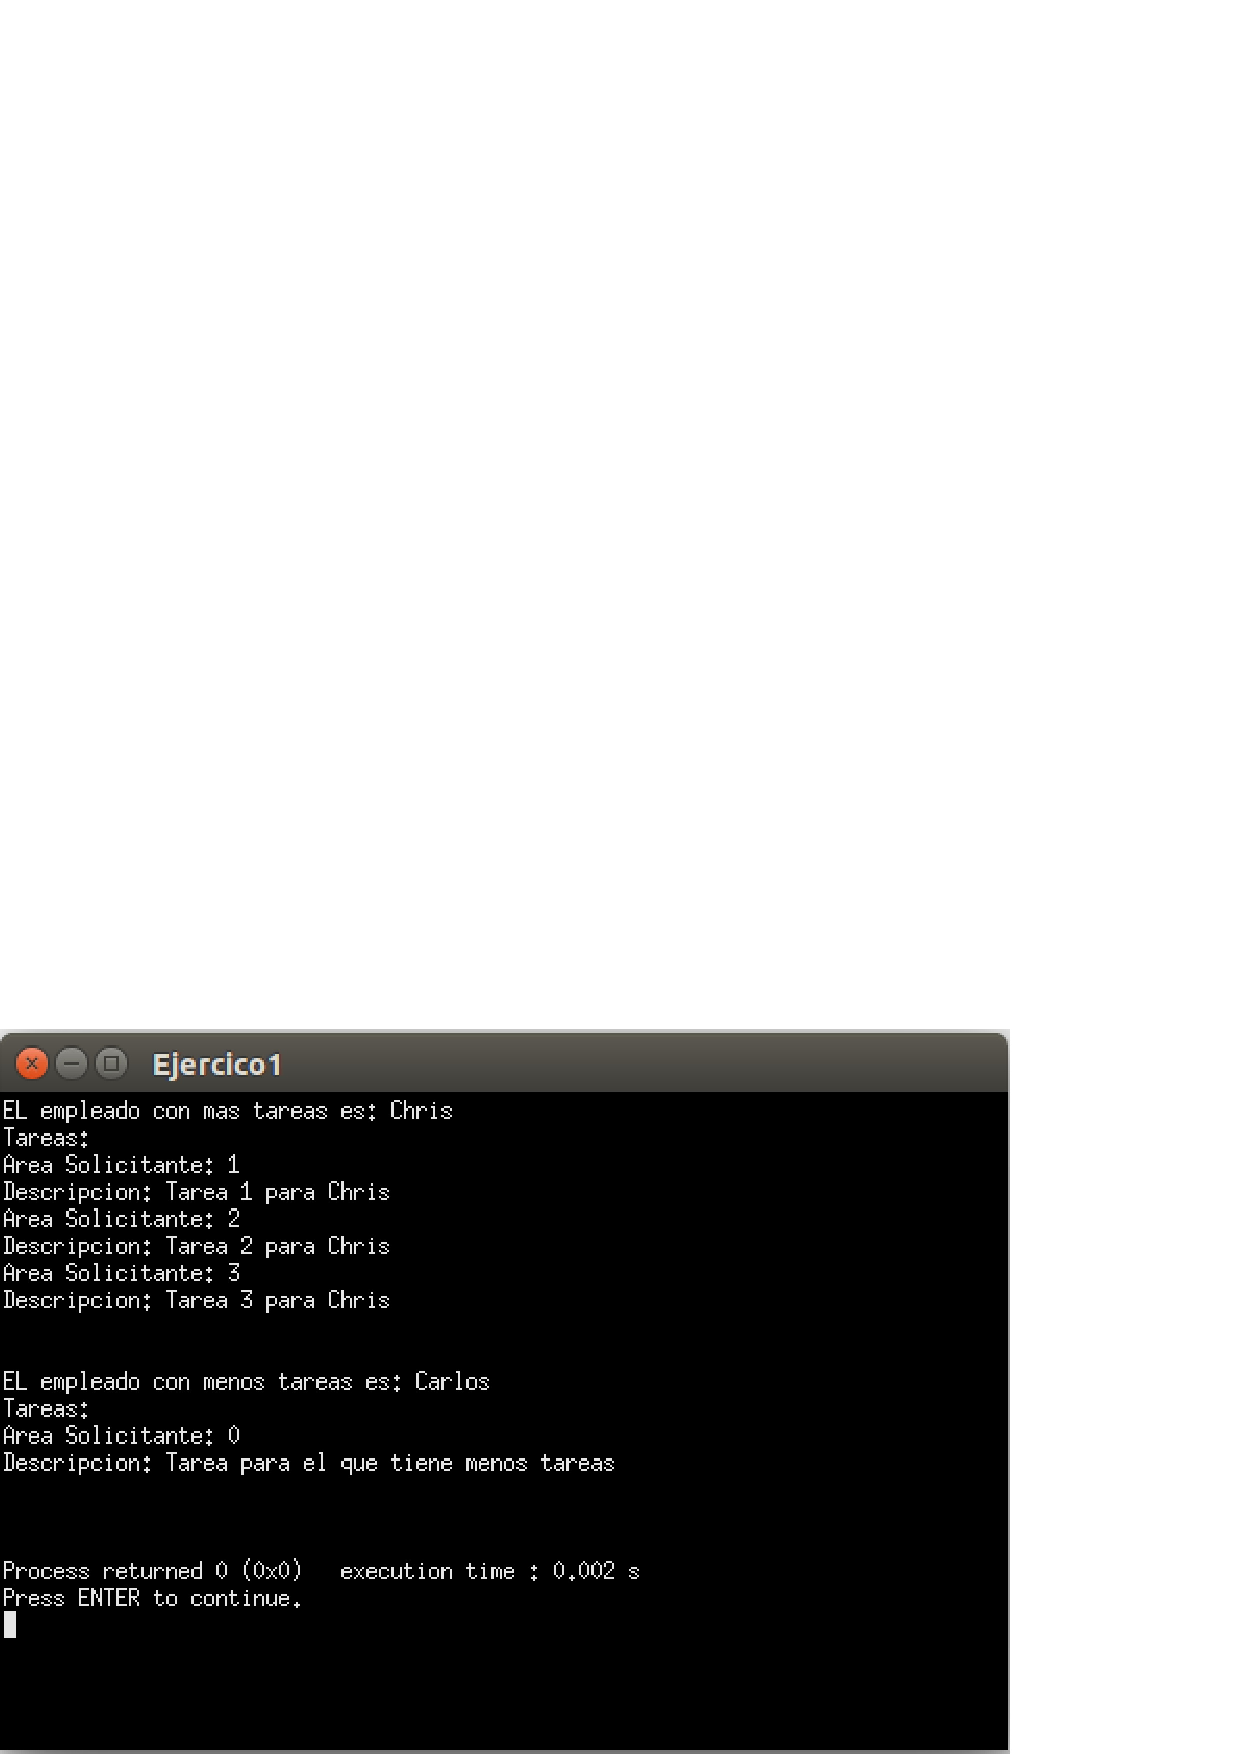
\includegraphics[scale=0.5]{1.png}
\end{figure}

 
\end{document}
